\chapter{Wykład 12. Zarządzanie zasobami ludzkimi w projekcie informatycznym}

\section{WBS i OBS}
% strona 20

\subsection*{Opracuj powiązane WBS i OBS dla projektu.}

\begin{enumerate}
\item Projekt informatyczny

\begin{enumerate}

\item Analiza

\begin{enumerate}

\item Systemu
\item Layoutu

\end{enumerate}
\item Projektowanie

\begin{enumerate}

\item Warstwa bazodanowa
\item Warstwa aplikacji
\item Warstwa prezentacji

\end{enumerate}
\item Implementacja

\begin{enumerate}

\item Warstwa bazodanowa
\item Warstwa aplikacji
\item Warstwa prezentacji

\end{enumerate}
\item Testowanie

\begin{enumerate}

\item Testy jednostkowe
\item Testy integracyjne
\item Testy funkcjonalne
\item Testy akceptacyjne
\item Testy wydajnościowe

\end{enumerate}
\item Wdrożenie

\begin{enumerate}

\item Zainstalowanie u klienta
\item Przeszkolenie użytkowników

\end{enumerate}
\item Utrzymywanie

\begin{enumerate}

\item Bieżące poprawianie błędów

\end{enumerate}
\end{enumerate}


\item Projekt informatyczny

\begin{enumerate}

\item Zarządzanie projektem

\begin{enumerate}

\item Plan projektu
\item Akceptacja wersji finalnej

\end{enumerate}

\item Projekt

\begin{enumerate}

\item Schemat bazy danych
\item Projekt graficzny
\item Diagramy UML
\item Instrukcja obsługi i konserwacji systemu

\end{enumerate}

\item Oprogramowanie

\begin{enumerate}

\item Warstwa bazodanowa
\item Warstwa aplikacji
\item Warstwa prezentacji

\end{enumerate}

\item Testy oprogramowania

\begin{enumerate}

\item Testy jednostkowe
\item Testy integracyjne
\item Testy funkcjonalne
\item Testy akceptacyjne
\item Testy wydajnościowe

\end{enumerate}

\item Dokumentacja

\begin{enumerate}

\item Instrukcja obsługi
\item Podręcznik użytkownika
\item Wyniki testów

\end{enumerate}

\item Wdrożenie

\begin{enumerate}

\item Wersja instalacyjnej (instalka)

\end{enumerate}
\end{enumerate}
\end{enumerate}

\clearpage

\subsection*{Przedstaw macierz RAM RACI dla projektu.}

R – odpowiedzialny, C – konsultowany, A – zatwierdzający, I – informowany

\begin{figure}[!h]
\centering
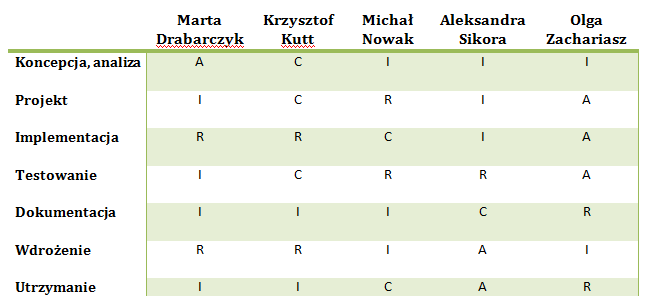
\includegraphics[width=1.1\textwidth]{macierzRAM.png}
\caption{Macierz RAM RACI dla projektu}
\label{fig:macierzRAM}
\end{figure}


% ===========================================================================

\section{Sposób wykorzystania integracji}
% strona 21

Zarządzanie integracją projektu zapewnia procesy, które mają za zadanie zapewnić, że elementy znajdujące się w procesie są koordynowane poprawnie. Do jego zadań należy też dokonywanie wyboru pomiędzy przewyższaniem oczekiwań a celami ich zaspakajania oraz wymaganiami ich udziałowców.
Do głównych procesów należą:

\begin{itemize}
\item tworzenie planu projektu,
\item wykonywanie planu projektu,
\item ogólny nadzór zmian.
\end{itemize}

Poszczególny proces działa wspólnie z innymi procesami, każdy z nich chociaż raz występuje we wszystkich fazach projektu.
Tworzymy plan projektu - zbiorczy dokument, który jest robiony na podstawie innych dokonanych rezultatów w procesach planowania. Używa się go jako przewodnika do tworzenia projektu jak również do jego kontrolowania.
Elementy przedstawienia planu projektów:

\begin{itemize}
\item karta projektu,
\item zakres,
\item zapis struktury pracy,
\item prowadzenie terminów i kosztów,
\item główne kamienie milowe oraz ich terminy,
\item główny lub wymagany personel,
\item główne czynniki ryzyka,
\item plan zakresu lub terminu,
\item trudne do rozwiązania problemy lub oczekujące na realizacje decyzje.
\end{itemize}

Inne elementy informacyjne zawiera się planie a jest to zależne od potrzeb i wymagań specyfiki projektu.
Wykonujemy plan projektu. Jest to podstawy proces który ma na celu realizację planu do którego wykorzystuje się większość zaplanowanego na projekt budżetu.
Nadzorujemy zmiany - proces związany z zmianami, które przynoszą oczekiwane korzyści przy wpływie na czynniki, zapewniają następowanie po sobie zmian i następnie ich zarządzeniem poprzez mierzenie stopnia realizacji, który ma na celu wpłynąć na wszystkie zmiany w planie, 
a następnie zmiany wpłyną na zasady.



% ===========================================================================

\section{Zasady stosowania pracy zdalnej}
% strona 29

textbf{I. Opracuj zasady stosowania pracy zdalnej (tele-pracy) w Twoim projekcie.}

Zasady stosowania pracy zdalnej w naszym projekcie:
\begin{itemize}
\item regularny przepływ informacji w obrębie zespołu wirtualnego,
\item komunikacja powinna odbywać się na bieżąco,
\item komunikaty powinny jasno przedstawiać pogląd na daną kwestie i  być poprzedzone wcześniejszymi uzgodnieniami,
\item każdy członek zespołu ma jasno określone zadanie,
\item pracujemy według określonego harmonogramu,
\item wszyscy członkowie zespołu muszą dotrzymywać terminów,
\item stosujemy oprogramowanie typu unified messaging - integrujące komunikację faksową, telefoniczną i e-mailową oraz pakiety wspierające pracę grupową,
\item używamy oprogramowania umożliwiającego przejmowanie zdalnej kontroli z domu nad komputerami znajdującymi się w biurze.

\end{itemize}


% ===========================================================================

\section{Zasady nagradzania}
% strona 46

Zasady nagradzania:

\begin{itemize}
\item docenianie wykonanej pracy,
\item należy większą wagę przykładać do sukcesów kolegów niż do ich porażek,
\item uznanie powinno być wygłoszone publicznie, tak aby inny członkowie zespołu je usłyszeli,
\item nagroda czy pochwała powinna być przekazana osobiście, a nie np. mailowo,
\item nagradzanie powinno mieć urozmaicone formy,
\item nagroda powinno zostać przyznana w miarę szybko,
\item osiągnięcia powinny kojarzyć się z nagradzaniem.
\end{itemize}
Nagradzanie może podnieść jakość wykonywanej pracy oraz zmobilizować zespół do jak najszybszego skończenia projektu. Natomiast głównym celem grupy projektowej jest uzyskanie pozytywnej oceny 
z przedmiotu, więc jakiekolwiek motywowanie będzie miało szanse oddziaływać do tego właśnie momentu.


% ===========================================================================

\section{Zasady motywowania}
% strona 72

W naszym zespole projektowym zostaną zastosowane następujące zasady motywacji:
\begin{itemize}
\item Motywowowanie poprzez pokazanie członkom zespołu, że ich wkład do projektu jest rzeczywisty i wykorzystywany
\item Wynagradzanie pracowników zgodnie z ich osiągnięciami
\item Jako korzyści brzegowe zastosujemy m.in. podział zysku, ubezpieczenie, możliwość dalszego rozwoju poprzez szkolenia zewnętrzne, różnego rodzaju karty umożliwiające darmową aktywność sportową, prywatna opieka zdrowotna
\item W naszej firmie będzie wykorzystywany głównie model Kierownika Y (kierownik typu X wprowadzany w sytuacjach krtycznych)
\item Zapewnienie dobrych warunków higienicznych zgodnie z teorią Herzberga, w celu uniknięcia obniżenia motywacji
\item Stosowanie różnych form premii oraz awansów
\item Publiczne pokazywanie uznania dla najlepszych pracowników
\item Zwiększanie odpowiedzialności w przypadku najlepszych pracowników
\item Dbanie o organizację pracy oraz dobre kontakty między pracownikami
\end{itemize}


% ===========================================================================

\section{Role w zespole projektowym}
% strona 83

\subsection*{Przeprowadź analizę Twojego zespołu projektowego pod względem ról w zespole.}

Role poszczególnym członkom zespołu zostały przydzielone na podstawie wyników testu przeprowadzonego na zajęciach.

\begin{figure}[!h]
\centering
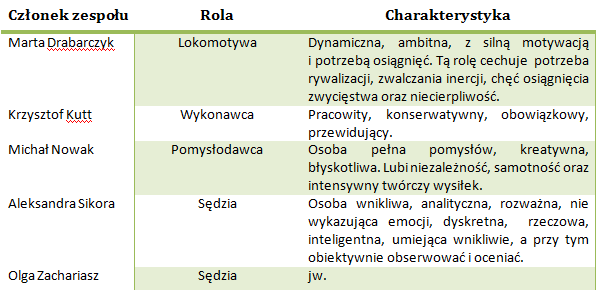
\includegraphics[width=1.1\textwidth]{roleWZespole.png}
\caption{Role w zespole projektowym}
\label{fig:roleWZespole}
\end{figure}

\subsection*{Przedstaw możliwe rozwiązania.}

Nasz zespół pod względem posiadania ról w zespole jest dość zróżnicowany, niemniej jednak dołączenie się osób posiadających role „koordynatora” czy też „duszy zespołu” byłoby dla nas plusem.


